\chapter{Etat de l'art}
\dochaptoc
\label{ch-chapter_2}

%
\section{La reconstruction : un problème d'inpainting}

\subsection{Contexte}


De nombreux problèmes en traitement de l'image consistent à corriger une région détériorée ou manquante et, suivant les situations, le masque spécifiant les zones manquantes est plus ou moins structuré. En retouche photographique, par exemple, le masque indiquant les régions à enlever d'une prise de vue~\cite{criminisi2004region} est fortement structuré et les structures sont fines (comme la grille visible à la figure~\ref{fig-inpainting-b}) ou grosses (personnages). Au contraire, le masque peut être très faiblement structuré et réparti, comme à la figure~\ref{fig-inpainting-e} où l'image est aléatoirement et partiellement acquise. Outre les situations où l'acquisition est volontairement lacunaire, les données peuvent souffrir de dysfonctionnements du capteur~\cite{zhang2013hyperspectral} et des bandes (resp. des pixels) peuvent être détériorés, conduisant à un masque fortement structuré et fin (resp. faiblement structuré et réparti).

Pour corriger ces défauts, de nombreuses méthodes proposées ces dernières décennies complètent les régions masquées en se basant sur l'information disponible et non-corrompue. Ainsi, les travaux de Bertalmio \etal{}~\cite{bertalmio2000image} se sont inspirés des techniques de restaurateurs en peinture employés par les musées et ont introduit le terme d'\emph{inpainting} pour désigner ces méthodes de complétion. Des exemples d'inpainting sont affichés aux \crefrange{fig-inpainting-a}{fig-inpainting-c} (resp. \crefrange{fig-inpainting-d}{fig-inpainting-f}) pour un masque structuré fin (resp. pour un masque réparti aléatoire). 

\begin{figure}[b]
    \centering
    \subfigure[\label{fig-inpainting-a}]{
        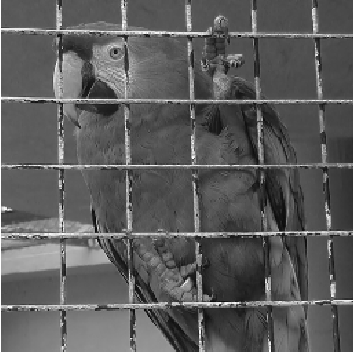
\includegraphics[width=0.25\textwidth]{img/chapitre2/figure1/initial-2.png}}\hspace{1em}
    \subfigure[\label{fig-inpainting-b}]{
        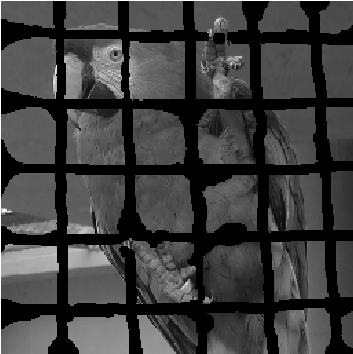
\includegraphics[width=0.25\textwidth]{img/chapitre2/figure1/mask-2.png}}\hspace{1em}
    \subfigure[\label{fig-inpainting-c}]{
        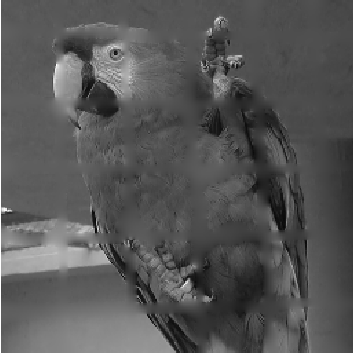
\includegraphics[width=0.25\textwidth]{img/chapitre2/figure1/final-2.png}}\\
    %
    \subfigure[\label{fig-inpainting-d}]{
        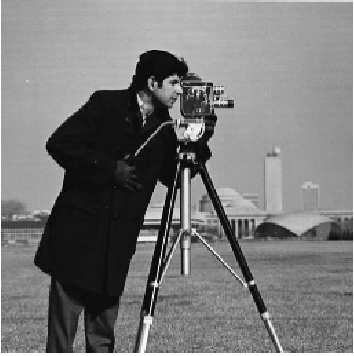
\includegraphics[width=0.25\textwidth]{img/chapitre2/figure2/initial.png}}\hspace{1em}
    \subfigure[\label{fig-inpainting-e}]{
        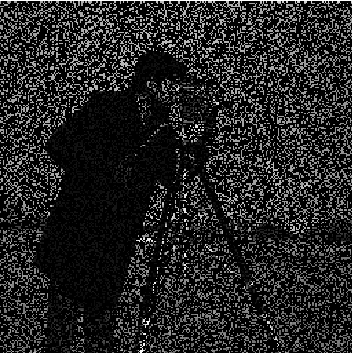
\includegraphics[width=0.25\textwidth]{img/chapitre2/figure2/mask.png}}\hspace{1em}
    \subfigure[\label{fig-inpainting-f}]{
        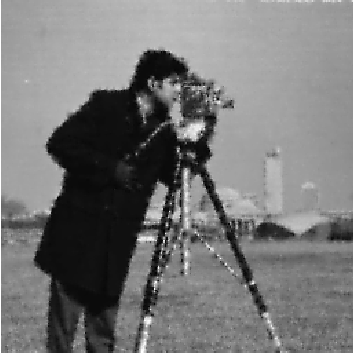
\includegraphics[width=0.25\textwidth]{img/chapitre2/figure2/final.png}}
    \caption{Exemple d'inpainting extrait de~\protect\cite{peyre2011numerical}. \protect\subref{fig-inpainting-a} Exemple d'image destinée à la retouche photographique. \protect\subref{fig-inpainting-b} Les pixels composant la grille sont masqués. \protect\subref{fig-inpainting-c} Résultat après inpainting. \protect\subref{fig-inpainting-d} Exemple d'acquisition complète. \protect\subref{fig-inpainting-e} La même image acquise partiellement. \protect\subref{fig-inpainting-f} Résultat après inpainting.
        \protect\label{fig-inpainting}} 
\end{figure}


La complétion peut être considérée comme un problème inverse dont le modèle d'acquisition est donné à la section suivante~\ref{subsec-direct-inverse-problem}. Plus largement, elle s'inscrit dans le cadre général de l'acquisition comprimée qui fournit des méthodes de restauration avec des garanties théoriques pour les problèmes inverses linéaires sous-déterminés. Les travaux d'Emmanuel Candès, Justin Romberg, Terence Tao et David Donoho~\cite{candes2006near, candes2006stable, donoho2006compressed} ont révolutionné le domaine du traitement du signal. Ceux-ci ont par exemple démontré qu'une image acquise avec une fréquence d'échantillonnage inférieure à celle de Nyquist pouvait être restaurée de manière exacte sous certaines conditions (dont une spécifiant que les données doivent être parcimonieuses dans une certaine base). Cette technique a été appliquée avec succès dans de nombreux domaines incluant l'\gls{irm}~\cite{boyer_algorithm_2014}, l'imagerie ultrasonique~\cite{quinsac_bayesian_2011}, l'astronomie~\cite{bobin_compressed_2008} ou la tomographie en microscopie~\cite{binev2012compressed, jacob2019MM, jacob2018MM}. %
%
Ces résultats ont rendu populaire les problèmes d'inpainting et il s'agit d'un domaine de recherche très actif en microscopie \gls{stem}~\cite{beche2016compressed,stevens2014potential} et \gls{sem}~\cite{anderson2013sparse} entre autres.


La technique d'inpainting est généralement associée à la reconstruction d'images 2D, mais elle s'étend au-delà pour les images multi-dimensionnelles dont une partie des voxels (l'équivalent des pixels pour une image multi-dimensionnelle) sont manquants.
%
La stratégie d'acquisition partielle décrite à la \cref{sec-ech-sensibles} s'inscrit dans ce contexte. En effet, la sonde ne visite qu'une partie de l'échantillon en suivant un chemin généralement aléatoire. Il en résulte des données spatialement sous-échantillonnées que les techniques d'inpainting peuvent compléter.
%
Notons également que ce schéma d'acquisition spatial ne s'accompagne pas d'un sous-échantillonnage spectral puisque, pour chaque position spatiale, le spectromètre \gls{eels} sépare simultanément toutes les pertes d'énergie conduisant à une acquisition complète du spectre. Il en résulte que le masque pour une telle stratégie est \emph{fortement structuré}.


\subsection{Modélisation du problème d'inpainting}\label{subsec-direct-inverse-problem}

Notons $\gls{Y}\in\mathbb{R}^{\gls{M}\times\gls{P}}$ la matrice qui correspondrait aux données \gls{eels} complètes composées de \gls{P} pixels et de \gls{M} canaux. 
%
Comme expliqué à la \cref{sec-ech-sensibles}, faire l'acquisition complète du spectre-image \gls{Y} n'est pas toujours possible dû à la détérioration introduite par le faisceau d'électron sur l'échantillon et c'est pourquoi un sous-échantillonnage spatial est envisagé, comme expliqué à la section~\ref{sec-positionnement-these}.
%
Ainsi, les spectres complets sont acquis en \gls{N} positions parmi \gls{P}, il en résulte un taux d'échantillonnage $\gls{r}=\gls{N}/\gls{P}$. L'ensemble des indices des \gls{N} positions spatiales visitées ainsi que la matrice d'observation sont respectivement notés \gls{I} et \gls{Yi}, où \gls{Yi} est la matrice de taille \taille{M}{N} rassemblant les $N$ colonnes de \gls{Y} indexées par \gls{I}. %

Nous avons vu à la \cref{sec-prop-eels} que le bruit présent dans les données est le mélange de plusieurs contributions avec chacune leur propriétés statistiques. Il en résulte que quantifier chacune de ces contribution est complexe en pratique et les modèles classiquement retenus dans la littérature sont les bruits poissonnien~\cite{egerton2011electron, mevenkamp2015poisson, stevens2018apl}, gaussien~\cite{stevens2014potential, binev2012compressed} et mixte poisson-gaussien~\cite{sanders2020inpainting}. Dans ce manuscrit, nous choisirons de modéliser la détérioration des données avec un bruit indépendant, additif et gaussien. Deux raisons motivent ce choix. D'abord, les paramètres du bruit sont difficiles à caractériser en pratique, si bien que le bruit gaussien plus simple est préféré. Ensuite, les expériences conduites à l'annexe~\ref{sec-bruit-mixte} avec un modèle de bruit mixte n'ont pas permis de mettre en évidence une perte de performances significative par rapport à un modèle gaussien seul. De plus, si une composante poissonnienne émerge particulièrement, des techniques de stabilisation de variance comme la transformée de Anscombe~\cite{anscombe1948transformation} permettent de \guillemets{convertir} le bruit mixte en un bruit gaussien.

Finalement, la matrice observée \gls{Yi} peut être décrite par le modèle suivant :
\begin{equation}
    \gls{Yi} = \gls{X}_{\gls{I}} + \gls{E}
\end{equation}
où \gls{X} est l'image idéle et \gls{E} est un terme résiduel représentant l'erreur de modèle et le bruit d'acquisition. Les éléments de \gls{E} sont supposés être indépendants et identiquement distribués selon une loi gaussienne centrée d'écart type \gls{sig}.

Le problème de reconstruction consiste à estimer un spectre-image de taille \taille{M}{P} complet (et possiblement débruité) \gls{X} à partir de \gls{Yi}. Cependant, cette tâche est mal posée puisque le nombre de paramètres \gls{P}\gls{M} est supérieur au nombre d'observations \gls{N}\gls{M} et la suite de ce chapitre étudiera les approches possibles pour résoudre ce problème inverse.


%
\section{Les différentes classes d'inpainting}

Cette section présente les méthodes de reconstructions classiquement rencontrées dans la littérature en les classant en cinq sections : les techniques d'interpolation, les techniques de \gls{mc} régularisés, les techniques par diffusion, les techniques par patch et les techniques par réseaux de neurones.


\subsection{Les techniques d'interpolation}\label{sec-interpolation}

\paragraph{Présentation du problème d'interpolation.} Le problème d'inpainting peut être vu comme un problème d'interpolation. L'image est alors définie par une fonction $f:\mathbb{R}^3\rightarrow \mathbb{R}$ associant chaque voxel $p\in\mathbb{R}^3$ à une valeur $f(p)\in\mathbb{R}$, connue en un ensemble de points $(s_k)_{k\in\gls{I}}$. Reconstruire l'image, c'est estimer les valeurs prises par $f$ sur un ensemble de points $(m_k)_{k\in \gls{I}^c }$ définis par le masque qu'il soit structuré ou non. 
%
Ce problème est facile en 1D et reste simple en dimension trois à condition que les points masqués soient répartis suivant une maille générée par trois ensembles de coordonnées $\mathcal{J}_x$, $\mathcal{J}_y$, $\mathcal{J}_{eV}$. L'interpolation est plus difficile dans le cas général, comme dans notre situation où le masque est aléatoirement et uniformément généré. L'espace doit alors être découpé en éléments de base, puis la fonction est interpolée sur ces éléments. Par exemple, en 2D, l'enveloppe convexe du nuage de points échantillonnés peut être découpée en un ensemble de triangles à l'aide de la triangulation de Delaunay présentée à l'annexe~\ref{abstr-voronoi-delaunay}. En particulier, chaque triangle de la triangulation a pour sommets des points du nuage et aucun point échantillonné ne se situe à l'intérieur du cercle circonscrit au triangle. L'avantage principale de cette triangulation sa faible complexité : $\mathcal{O}(|\gls{I}|\log |\gls{I}|)$~\cite{lee1980two}, voire $\mathcal{O}(|\gls{I}|\log \log |\gls{I}|)$~\cite{dwyer1987faster} dans de nombreux cas.

\paragraph{Interpolation par \Glsentrylong{ppv}.} L'interpolation par \gls{ppv} est la technique d'interpolation la plus simple et la moins coûteuse. Elle consiste à associer à chaque point à interpoler la valeur prise par $f$ au point échantillonné $s_{k}$ le plus proche. Cela consiste à associer $f(s_{k})$ à tout point $x$ appartenant à la cellule de Voronoi de $s_{k}$, définie par l'ensemble des points plus proches de $s_k$ que de tout autre point de $(s_{k'})_{k'\neq k}$. Le diagramme de Voronoi constitué de l'ensemble des cellules est décrit à l'annexe~\ref{abstr-voronoi-delaunay} et a la même complexité que la triangulation de Delaunay. Cette méthode, bien que très peu coûteuse, est aussi la moins efficace puisque la fonction interpolée est constante par morceaux, ce qui entraîne une erreur de reconstruction élevée. Cela est particulièrement visible sur l'exemple d'interpolation \gls{ppv} donné aux figures \ref{fig-interpolation-a} et \ref{fig-interpolation-d} puisque les cellules de Voronoi apparaissent clairement sur l'image.

Pour lisser davantage la fonction interpolée, une solution consiste à associer au point à interpoler $x$ une pondération des valeurs prises par les points $(s_k)_k$ voisins, c'est-à-dire
\begin{equation}\label{eq-weighted-interp}
    \hat{f}(x) = \sum_{k\in\gls{I}} w_k(x) f(s_k)
\end{equation}%
\begin{marginfigure}%
    \centering
    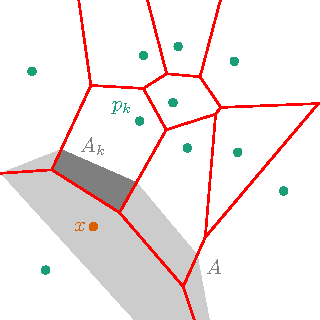
\includegraphics[]{img/chapitre2/figure3/Voronoi_Natural.pdf}
    \caption{Illustration de la méthode par plus proches voisins naturels. Le diagramme de Voronoi associé à l'ensemble de points $(s_k)_k$ connu (en vert) est affiché (en rouge). Lorsque le nouveau point (en orange) est ajouté, une cellule (en gris) est ajoutée au diagramme.}
    \label{fig-natural-weight}
\end{marginfigure}%
\noindent où $w_k(x)$ est le poids de $x$ associé au point échantillonné $s_k$ (la somme des poids vaut 1). Une approche classique consiste à évaluer le diagramme de Voronoi de $(s_k)_{k\in\gls{I}}$ (en rouge à la \cref{fig-natural-weight}), puis une deuxième fois en ajoutant $x$ (la cellule supplémentaire est en gris à la \cref{fig-natural-weight}). Si l'on note $A_k$ l'aire de l'intersection entre cette nouvelle cellule et la cellule précédemment associée à $s_k$ et $A$ l'aire de la nouvelle cellule associée à $x$, alors on pose $w_k(x)=A_k/A$. Cette approche, appelée interpolation par plus proches voisins naturels~\cite{sibson1981interpreting,cazals2006delaunay}, donne de meilleurs résultats que l'interpolation par plus proche voisins, mais elle est aussi plus lourde d'un point de vue calculatoire.

\paragraph{Interpolation pour des ordres supérieurs.} Comme expliqué plus haut, l'interpolation dans le cas multidimensionnel est généralement réalisée en ajustant une fonction d'ordre fixe sur chaque simplexe issu de la triangulation de Delaunay. Ainsi, l'interpolation \gls{ppv} ajuste une fonction constante par morceau sur les sommets du simplexe. Des ordres supérieurs peuvent être utilisés, comme l'interpolation linéaire ou cubique en 1D correspondant respectivement à des fonctions d'ordre 1 et 3. En 2D, cela consiste à ajuster des plans ou des surfaces cubiques par régression aux sommets du triangle. En plus grande dimension, l'interpolation linéaire est réalisée par interpolation barycentrique~\cite{hormann2014barycentric}. Les figures~\ref{fig-interpolation-b}, \ref{fig-interpolation-c}, \ref{fig-interpolation-e} et \ref{fig-interpolation-f} permettent de visualiser le résultat de la régression dans les cas linéaire et cubique.
  
\begin{figure}[h]
    \centering
    \subfigure[\label{fig-interpolation-a}\gls{ppv}]{
        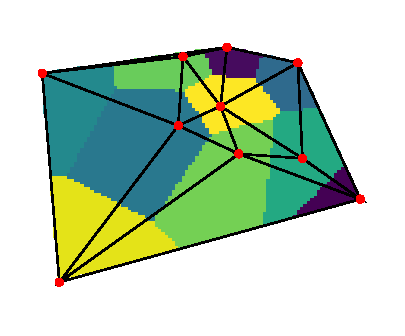
\includegraphics[width=0.29\textwidth]{img/chapitre2/figure4/nearest.pdf}}\hspace{1em}
    \subfigure[\label{fig-interpolation-b}Interpolation linéaire]{
        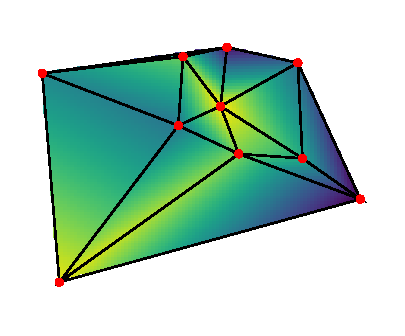
\includegraphics[width=0.29\textwidth]{img/chapitre2/figure4/linear.pdf}}\hspace{1em}
    \subfigure[\label{fig-interpolation-c}Interpolation cubique]{
        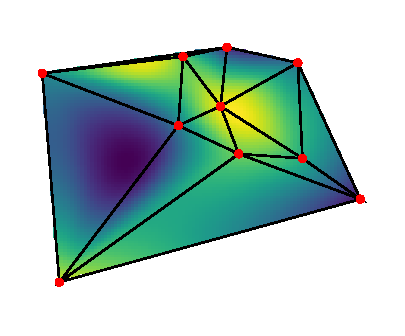
\includegraphics[width=0.29\textwidth]{img/chapitre2/figure4/cubic.pdf}}\\
    \subfigure[\label{fig-interpolation-d}\gls{ppv}]{
        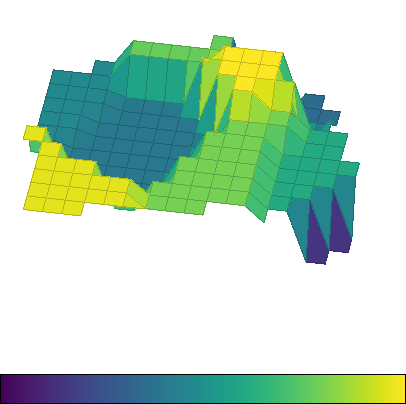
\includegraphics[width=0.29\textwidth]{img/chapitre2/figure4/surf_nearest.pdf}}\hspace{1em}
    \subfigure[\label{fig-interpolation-e}Interpolation linéaire]{
        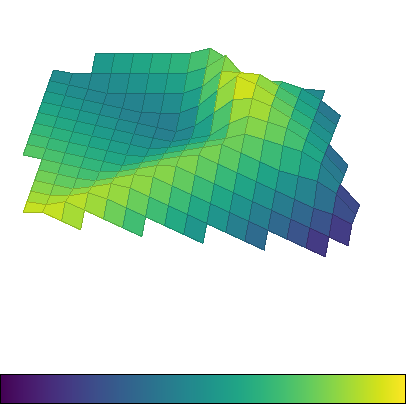
\includegraphics[width=0.29\textwidth]{img/chapitre2/figure4/surf_linear.pdf}}\hspace{1em}
    \subfigure[\label{fig-interpolation-f}Interpolation cubique]{
        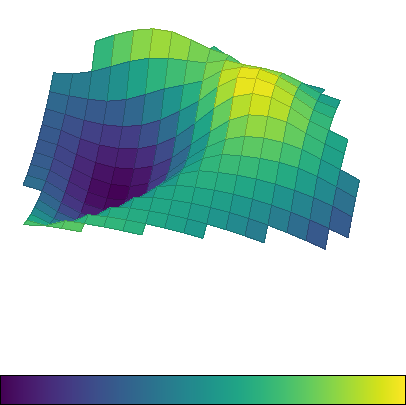
\includegraphics[width=0.29\textwidth]{img/chapitre2/figure4/surf_cubic.pdf}}
    \caption{Exemple d'interpolation sur un nuage de points aléatoirement généré (en rouge). La fonction est interpolée sur l'enveloppe convexe en s'appuyant sur la triangulation de Delaunay représentée en noir. \protect\subref{fig-interpolation-a} Interpolation \gls{ppv}. \protect\subref{fig-interpolation-b} Interpolation linéaire. \protect\subref{fig-interpolation-c} Interpolation cubique. Les fonctions interpolées sont également représentées dans le même ordre sous forme de surfaces aux figures~\subref{fig-interpolation-d} à \subref{fig-interpolation-f} (la résolution spatiale est diminuée pour des raisons d'affichage).
        \protect\label{fig-interpolation}}
\end{figure}


\paragraph{Avantages et inconvénients.} Les méthodes d'interpolation ont pour principal avantage leur faible complexité et leur rapidité, ce qui en font des méthodes populaires en reconstruction en ligne~\cite{sibson1981interpreting, cazals2006delaunay, trampert2018ultramicroscopy}. Néanmoins, elles ne sont pas robustes puisqu'elles s'ajustent aux valeurs disponibles elles-mêmes corrompues. Elles ne permettent pas d'introduire plus d'information a priori que l'ordre de la fonction à interpoler.

\subsection{Les techniques par \glsentrylong{mc} régularisés}\label{sec-MC-regul}

Une approche \emph{variationelle} en inpainting est une méthode calculant l'image reconstruite en minimisant une fonction objectif. En particulier, une technique par \gls{mc} régularisés fournit une image reconstruite \gls{Xh} en résolvant le problème de minimisation suivant~\cite[Section~6.3]{boyd2004convex}
\begin{equation}\label{eq-MC-regul}
    \gls{Xh} = \argmin_{\gls{X}} \frobnorm{\gls{X}_{\gls{I}} - \gls{Yi}} + \lambda \mathcal{R}(\gls{X})
\end{equation}
où $\frobnorm{\gls{X}_{\gls{I}} - \gls{Yi}}$ est le terme d'attache aux données et où l'opérateur $\mathcal{R}$ est une régularisation. Le scalaire $\lambda$ permet d'ajuster l'importance de la régularisation par rapport au terme d'attache aux données. Cette formulation peut s'interpréter comme (si on choisi le paradigme bayésien) l'estimateur du \gls{map} puisque la formule de Bayes donne la fonction de vraisemblance $P(\gls{X}|\gls{Yi}) \propto P(\gls{Yi}|\gls{X}) P(\gls{X})$. En considérant l'opposé de la log-vraissemblance, l'estimée est l'image \gls{X} minimisant la fonction
\begin{equation}
    -\log P(\gls{X}|\gls{Yi}) \propto
    \underbrace{-\log P(\gls{Yi}|\gls{X})}_{\frobnorm{\gls{X}_{\gls{I}} - \gls{Yi}}}
    \underbrace{- \log P(\gls{X})}_{\mathcal{R}(\gls{X})}.
\end{equation}
Il en résulte que le terme d'attache aux données est choisi en fonction du modèle statistique du bruit tandis que la régularisation dépend de l'information a priori disponible pour \gls{X}. Ces méthodes gèrent donc mieux la connaissance du bruit que les techniques d'interpolation et sont ainsi plus robustes. En particulier, le terme d'attache aux données pour un bruit additif gaussien blanc est la fonction coût \gls{mc} $\frobnorm{\gls{X}_{\gls{I}} - \gls{Yi}}$. D'autres fonctions peuvent être utilisés lorsque la statistique du bruit est différente, comme la norme $\ell_1$ pour un bruit laplacien~\cite{frecon2017bayesian} ou la divergence de Kullback–Leibler pour un bruit poissonnien~\cite{ono2013poisson}. Notons encore que les problèmes de \gls{mc} régularisés conviennent que le masque soit structuré ou non et qu'ils sont également utilisés pour la complétion en se basant sur une triangulation, comme c'est le cas en ajustement de surface~\cite{zhong2016surface,cazals2006delaunay}.

Un choix particulièrement classique pour la régularisation est la fonction quadratique $\mathcal{R}(\gls{X}) = \frobnorm{\gls{X}}$, on parle alors de régularisation de Tikhonov. L'avantage de cette forme est que la solution est  donnée par une expression mathématique directe, ne nécessitant qu'une inversion de matrice. La loi a priori de \gls{X} est gaussienne centrée et promeut des données d'amplitude bien répartie autours de la moyenne.

Les techniques de \gls{mc} régularisés sont également d'un intérêt particulier dans le cas de données  parcimonieuses, c'est-à-dire dont la proportion d'entrées non nulles est faible. Dans ce cas, la régularisation idéale est la pseudo-norme $\ell_0$ \footnote{La pseudo-norme $\ell_0$ de \gls{X} vaut le nombre d'entrées non-nulle de \gls{X}. Il ne s'agit pas d'une norme puisque $||\alpha\gls{X}||_0 = ||\gls{X}||_0$ pour tout scalaire $\alpha$ non nul.} puisque celle-ci contraint le nombre d'éléments non-nuls. Malheureusement, résoudre ce problème d'estimation est très compliqué en pratique puisque la norme $\ell_0$ n'est pas convexe et on lui préfère généralement sa relaxation convexe : la norme $\ell_1$ définie par $||\gls{X}||_1 = \sum |\gls{X}_{ij}|$. Cette méthode est souvent appelée Lasso~\cite{tibshirani1996regression} de l'acronyme \emph{least absolute shrinkage and selection operator}. Enfin, il faut noter qu'utiliser la norme $\ell_1$ comme régularisation biaise le résultat. Pour corriger cela, des travaux ont proposé de résoudre le problème inverse en deux temps. D'abord, la technique Lasso est appliquée afin de déterminer les entrées non-nulles de l'estimée. Ensuite, une régression des moindres carrés est réalisée sur ce support. Cette méthode en deux temps est appelée post-LS (pour Least Square) ou encore \emph{refitting}~\cite{belloni2013least, lederer2013trust, deledalle2017clear}.

Utiliser une norme de $\gls{X}$ comme régularisation n'est pas toujours adaptée à l'information a priori disponible,  et l'on préfère généralement pénaliser $\mathcal{A}\gls{X}$ où $\mathcal{A}$ est un opérateur linéaire adapté. Ainsi, une alternative très populaire en traitement du signal consiste plutôt à contraindre le gradient de l'image $\nabla\gls{X}$, conduisant à une régularisation $\mathcal{R}(\gls{X})=\frobnorm{\nabla\gls{X}}$, on parle aussi d'énergie de Sobolev. Cela produit une image lissée. De même, la régularisation $\ell_1$ peut être couplée avec un opérateur linéaire $\mathcal{A}$ pour favoriser la parcimonie du signal dans un cas particulier, par exemple :
\begin{itemize}
    \item si $\mathcal{A}$ est un changement de base telle que $\mathcal{A}\gls{X}$ soit parcimonieuse, la régularisation $||\mathcal{A}\gls{X}||_1$ est adaptée,
    \item si $\mathcal{A}$ est l'opérateur de gradient spatial discret $\nabla$, la régularisation $||\nabla \gls{X}||_1$ appelée \gls{tv} promeut une image ayant peu de contours (l'image résultante est constante par morceaux).
\end{itemize}


\subsection{Les techniques par diffusion}

La diffusion est un processus physique intuitif tendant à équilibrer les différences de concentration au sein d'un fluide sans créer ou détruire de masse. Ce phénomène est régi par l'équation de diffusion suivante
\begin{equation}
    \frac{\partial u}{\partial t} \triangleq \dot{u}(x, y, t) = \mathrm{div} (D(x, y)\cdot \nabla u)
\end{equation}
où $u$ est la concentration, $D$ est le coefficient de diffusion et $\nabla$ est l'opérateur gradient. En traitement de l'image, on identifie la concentration avec la valeur en niveau de gris prise en une position particulière. Si le coefficient de diffusion est constant sur toute l'image, on parle de diffusion \emph{isotrope}, sinon, on parle de diffusion \emph{anisotrope}.

La technique de diffusion la plus simple est la diffusion isotrope en débruitage, conduisant au problème aux dérivées partielles suivant\footnote{Cette équation correspond aussi à l'équation de la chaleur dans le cas où il n'y a pas de source de chaleur.}
\begin{align}
&\dot{u} = D \cdot \Delta u\\
&u(\cdot, t=0) = y
\end{align}
où $\Delta$ est l'opérateur de laplacien spatial discret et $y$ est l'image bruitée. Ce problème est équivalent à un filtrage avec un noyau gaussien d'écart-type $\sqrt{2t}$\footnote{L'image resultante en diffusion n'est pas l'image $u(\cdot, t=\infty)$ puisque celle-ci est constante (la diffusion tend à égaliser les niveaux de gris). Il faut choisir un instant $t^*$ où arrêter la trajectoire et l'image resultante est $u(\cdot, t^*)$.} \cite{weickert1998anisotropic}. Le problème de cette technique est que la diffusion introduit un flou sur les contours de l'image. C'est pourquoi Perona et Malik~\cite{perona1990scale} ont proposé la diffusion anisotropique pour préserver les contours de l'image. Le coefficient de diffusion est diminué au niveau des contours tandis qu'il reste élevé au sein de zones homogènes. Le problème résultant s'écrit
\begin{align}
    &\dot{u}(x, y, t) = \mathrm{div} (D(|\nabla u|^2)\cdot \nabla u)\\
    & D(s) = \frac{1}{1+s^2/\lambda^2} \quad \text{pour $\lambda > 0$}
\end{align}

La technique de diffusion ne suffit cependant pas pour l'inpainting puisque la structure n'est pas propagée et un transport de matière doit être ajouté. Les travaux de Bertalmio \textit{et al.}~\cite{bertalmio2000image} ont été pionniers dans ce domaine et ont été à l'origine du terme \emph{inpainting}. S'inspirant des techniques de restauration en art, ils ont envisagé une technique par transport de matière propageant l'information le long de lignes de niveau (les lignes reliant les points de l'image ayant le même niveau de gris) dans le cas où le masque est structurée. Un terme de diffusion anisotrope était ajouté afin d'éviter que les lignes de niveau ne se croisent. D'autres techniques basées sur la variation totale on suivi~\cite{shen2002mathematical, chan2001nontexture} mais le principe fondamental consiste à propager la structure.

Ces techniques sont très bien adaptées aux images pour lesquelles le masque est très structurée, mais elles ne conviennent pas lorsque l'information est répartie. En effet, ces techniques reposent sur la propagation de contour. Dans le cas où les données sont réparties, aucun contour ne peut être propagé. C'est pourquoi nous n'utiliserons pas ces méthodes dans ce manuscrit.


\subsection{Les techniques par patch}\label{sec-art-patch}

Une extension des méthodes variationelles exploite la redondance spatiale dans l'image (la figure~\ref{fig-redondance-spatiale-search} illustre cette propriété), on parle alors de \emph{méthode par patch} ou \emph{examplar-based}. Elles constituent un ensemble de méthodes très populaires et performantes dont l'intérêt n'a cessé de grandir ces dernières décennies afin de résoudre des problèmes inverses comme le débruitage, l'inpainting ou la déconvolution.

\begin{figure}
    \centering
    \subfigure[\label{fig-redondance-spatiale-search}]{
        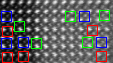
\includegraphics[width=0.7\textwidth]{img/chapitre2/figure5/search.png}}\\
    \subfigure[Atome rouge\label{fig-redondance-spatiale-dic1}]{
        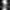
\includegraphics[width=0.25\textwidth]{img/chapitre2/figure5/dico_red.png}}\hfill
    \subfigure[Atome vert\label{fig-redondance-spatiale-dic2}]{
        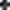
\includegraphics[width=0.25\textwidth]{img/chapitre2/figure5/dico_green.png}}\hfill
    \subfigure[Atome bleu\label{fig-redondance-spatiale-dic3}]{
        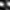
\includegraphics[width=0.25\textwidth]{img/chapitre2/figure5/dico_blue.png}}
    \caption{Illustration de la redondance spatiale en imagerie haute résolution. Une image \gls{haadf} est affichée à la figure~\subref{fig-redondance-spatiale-search} et trois familles de patch sont représentées en rouge, vert et bleu. Les patchs appartenant à une famille donnée sont tous semblables bien que éloignés dans l'image, confirmant l'hypothèse selon laquelle le contenu spatial de l'image est redondant. Les trois premiers atomes d'un dictionnaire appris à l'aide de la méthode mini-batch~\cite{mairal2009online} sont représentés aux figures~\subref{fig-redondance-spatiale-dic1} à \subref{fig-redondance-spatiale-dic3} et correspondent respectivement aux familles de patchs rouge, verte et bleue.
        \protect\label{fig-redondance-spatiale}}
\end{figure}

Ces méthodes sont à opposer aux techniques dites \emph{locales} où une valeur est corrigée en ne la comparant qu'avec son voisinage, comme lorsqu'une image est convoluée avec un masque gaussien en débruitage. Le premier exemple de méthode \emph{non-locale} a été l'algorithme de débruitage Non-Local Means~\cite{buades2005non} qui recherche des patchs semblables dans l'image afin de moyenner les pixels centraux. Par exemple, si l'on considère une famille de patchs de la figure~\ref{fig-redondance-spatiale-search}, les pixels centraux de chacun de ses membres peuvent être débruités en les substituant par leur moyenne. D'autres techniques plus évoluées en débruitage ont suivi, parmi lesquelles Block Matching and 3D filtering (BM3D)~\cite{dabov2007image} et Non Local Bayes~\cite{lebrun2013nonlocal}. Cependant, reconstruire de manière non-locale ne peux se faire naïvement que si le masque est structurée. Par exemple, l'algorithme \gls{ebi}~\cite{criminisi2004region} reconstruit des images partiellement corrompus en remplaçant de manière itérative les patchs manquants par le patch entier lui ressemblant le plus dans la zone connue. Des résultats ont également exprimé Non-Local Means sous forme variationnelle, permettant ainsi des applications en reconstruction d'images dont l'information est répartie~\cite{peyre2008non, unni2018non, arias2009variational, yang2012nonlocal}.

Pour imposer la redondance spatiale, des algorithmes performants cherchent à représenter les patchs de l'image de manière parcimonieuse à l'aide d'\emph{atomes}\footnote{Ici, on ne parle pas des composants élémentaires de la matière, mais bien des patchs constituant le dictionnaire.} contenus dans un \emph{dictionnaire}, on parle alors de méthode par \gls{ad}. Une formulation générique de cette technique peut s'écrire comme le problème d'optimisation suivant~\cite{mairal2009online}
\begin{equation}
    \begin{aligned}
    (\mathbf{D}^*,\mathbf{A}^*) = &\argmin_{(\mathbf{D}, \mathbf{A})}
    \frac{1}{2} \frobnorm{ \mathbf{R}(\gls{Y}) - \mathbf{D A}} + \lambda  || \mathbf{A} ||_1\\
    &\text{tel que } || \mathbf{D}_k ||_2 = 1 \quad \forall k\\
    \end{aligned}
\end{equation}
où $\mathbf{D}$ et $\mathbf{A}$ sont les matrices contenant respectivement les atomes et la décomposition parcimonieuse associé à chaque patch (on parle aussi de \emph{code}). $\mathbf{R}$, quant à lui, est l'opérateur permettant d'extraire les patchs des données et l'image reconstruite est obtenue par $\mathbf{R}^*(\mathbf{D}^*\mathbf{A}^*)$ où $\mathbf{R}^*$ est un pseudo inverse de $\mathbf{R}$. La contrainte permet de normaliser les atomes tandis que la régularisation $|| \mathbf{A} ||_1$ contraint le code à être parcimonieux. 
%
La \cref{fig-redondance-spatiale} donne un exemple d'application de cette méthode pour une image \gls{haadf} haute-résolution, les trois premiers atomes étant affichés sur les figures~\ref{fig-redondance-spatiale-dic1} à \ref{fig-redondance-spatiale-dic3}.
%

%
Cependant, la difficulté de cette approche est que la fonctionnelle à minimiser est non-convexe, si bien que l'on se contente couramment d'un résultat non-équivalent et sous-optimal en alternant l'estimation du code et l'apprentissage du dictionnaire dont les formulations isolées sont convexes.
%
D'une part, si le dictionnaire $\mathbf{D}$ est fixé, l'estimation du code $\mathbf{A}$ consiste à obtenir une représentation parcimonieuse en résolvant 
\begin{align}
    \mathbf{A}^{opt} = &\argmin_{\mathbf{A}} \frobnorm{ \mathbf{R}(\gls{Y}) - \mathbf{DA}}\\
    &\text{tel que}
    \quad
    ||\mathbf{A}_i||_0 \leq N_{\mathrm{max}}\quad\forall i
\end{align}
où $N_{\mathrm{max}}$ est le nombre maximal d'atomes autorisés pour décrire un patch. Orthogonal Matching Pursuit (OMP)~\cite{mallat1993matching, pati1993orthogonal} est un algorithme glouton qui tente d'approximer la solution de ce problème NP-difficile. Son principe consiste à sélectionner le meilleur atome du dictionnaire à chaque itération, à savoir celui qui maximise son produit scalaire avec le résidu, puis à mettre à jour le résidu en appliquant une projection orthogonale du signal que l'on souhaite approximer sur l'espace vectoriel engendré par les atomes précédemment sélectionnés. Cette orthogonalisation est importante puisqu'elle stabilise et accélère la convergence de cet algorithme glouton.
%
D'autre part, une fois l'étape de recherche du code réalisée, le dictionnaire $\mathbf{D}$ doit être mis à jour en conservant $\mathbf{A}$ fixe, non pas en une étape, mais en améliorant chaque atome successivement afin d'alléger le coût. Plus précisément, l'atome $\mathbf{D}_k$ est mis à jour en déterminant le résidu $\mathbf{E}_k$ obtenu en soustrayant la contribution de tous les autres atomes $(\mathbf{D}_{k'})_{k'\neq k}$  des données $\mathbf{R}(\gls{Y})$ et en ne conservant que les patchs utilisant l'atome $\mathbf{D}_k$ dans leur code. La mise à jour de l'atome est enfin réalisée en déterminant le vecteur $\hat{\mathbf{d}}$ résolvant
\begin{equation}\label{eq-dico-ksvd}
    (\hat{\mathbf{a}}, \hat{\mathbf{d}}) = \argmin_{\mathbf{a}, \twonorm{\mathbf{d}}=1} \frobnorm{\mathbf{E}_k-\mathbf{da}}.
\end{equation}
Le code précédemment fixé est mis à jour à l'aide des coefficients corrigé $\hat{\mathbf{a}}$ avant de poursuivre l'amélioration du dictionnaire. L'approximation de rang un donnée à l'équation~\eqref{eq-dico-ksvd} est réalisée en appliquant une SVD tronquée à $\mathbf{E}_k$. La répétition des deux étapes, apprentissage du code par OMP et amélioration du code par SVD, constitue la méthode K-SVD utilisée en débruitage d'images~\cite{elad2006image}.

Toutefois, cette approche contraint le bruit à être uniforme, puisque l'algorithme OMP fait l'hypothèse intrinsèque que le bruit a une structure de sphère dans l'espace des patchs. Pour corriger cela, Mairal \etal{}~\cite{mairal2008tip} ont proposés la construction d'un vecteur $\beta$ de même taille que l'image constitué de poids pour chaque voxel
\begin{equation}
    \beta_p = \frac{\min_{p'\in\text{image}}\sigma_{p'}}{\sigma_p}
\end{equation}
où $\sigma_p>0$ désigne l'écart-type du bruit associé au voxel $p$. L'algorithme OMP est ensuite corrigé en définissant un nouveau produit scalaire dans l'espace des patchs. Plus précisément, chaque élément de cet espace est pondéré par les poids associés au patch courant avant d'appliquer le produit scalaire euclidien. De même, le terme $\mathbf{E}_k-\mathbf{da}$ de l'approximation de rang un à l'équation~\eqref{eq-dico-ksvd} est pondéré à l'aide de ces poids, conduisant à une approximation de rang un pondérée plus complexe. 
%
Cette correction peut être étendue au problème d'inpainting avec un masque faiblement structuré en supposant un bruit de puissance infinie (\ie{} $\sigma_p=\infty$) pour les pixels manquants et en fixant un niveau de bruit constant ailleurs. Ainsi, les pixels manquants se voient affectés d'un poids $\beta_p$ nul, conduisant à des versions masquées de OMP et de l'approximation de rang un. Cette technique pondérée est appelée \gls{wksvd}.

Le problème principal de wKSVD est sa complexité algorithmique, principalement due à la SVD requise par l'étape de mise à jour du dictionnaire. C'est pourquoi l'algorithme \gls{itkrmm}~\cite{naumova2018fast, naumova2017dictionary} a pris le contre-pied en proposant une approche plus rapide ne nécessitant pas de SVD. Elle repose sur l'hypothèse que les données corrompues sont parcimonieuses non pas dans le dictionnaire $\mathbf{D}$ mais plutôt dans une version corrompue du dictionnaire dont le masque dépend du patch considéré et résout le problème comme wKSVD en alternant choix du code et mise à jour du dictionnaire.
%
L'estimation du code est réalisée par seuillage, en ne conservant pour chaque patch que les $N_\mathrm{max}$ atomes corrompus dont le produit scalaire avec les données masquées est maximal. 
La mise à jour du dictionnaire est ensuite réalisée en calculant pour chaque atome la moyenne des résidus sur l'ensemble des patchs corrompus, puis en les normalisant. 
%
Ces travaux soulignent également le besoin de soustraire une composante faible-rang des données afin d'éviter que le dictionnaire soit mal conditionné et que la plupart des atomes soient distordus en direction de la composante faible-rang. C'est pourquoi cette composante est intégrée dans le calcul des résidus, mais sa contribution est soustraite des atomes avant la normalisation lors de la mise à jour du dictionnaire, afin que le dictionnaire soit orthogonal à l'élément faible-rang.

Finalement, d'autre travaux préfèrent avoir recours à des modèles bayésiens afin de déterminer $\mathbf{D}$ et $\mathbf{A}$ à partir des données corrompues. Un algorithme très populaire en microscopie est \gls{bpfa}~\cite{xing2012siam} qui a été conçu initialement pour l'imagerie hyperspectrale. Une description succincte du modèle est donnée ci-dessous tandis que le détail complet est disponible dans~\cite{xing2012siam}. Les atomes $\mathbf{D}_k\in\mathbb{R}^n$ et le bruit $\mathbf{B}$ sont supposés suivre des lois gaussiennes indépendantes tandis que les lignes $\mathbf{A}_{i, :}$ de $\mathbf{A}$ suivent une construction beta-bernouilli. Le modèle hiérarchique complet de BPFA est
\begin{equation}\label{eq-BPFA-model}
\begin{aligned}
    &\mathcal{R}(\gls{Y}) = \mathbf{D A + B} 
    &&\mathbf{E}_i\sim\mathcal{N}(0, \gamma_\mathbf{E}^{-1}\mathcal{I}_n)\\
    %
    &\mathbf{D} = [\mathbf{D}_1, \dots, \mathbf{D}_K]
    &&\mathbf{D}_k\sim\mathcal{N}(0, n^{-1}\mathcal{I}_n)\\
    %
    &\mathbf{A}_{i, :} = \mathbf{Z}_{i, :}\cdot \mathbf{W}_{i, :}
    &&\mathbf{W}_{i, :}\sim\mathcal{N}(0, \gamma_\mathbf{W}^{-1}\mathcal{I}_K)\\
    %
    &\mathbf{Z}_{i, :}\sim \prod_{k=1}^{K}\mathrm{Bernouilli}(\pi_k)
    &&\pi_k\sim\mathrm{beta}\left( \frac{a}{K}, b\frac{K-1}{K} \right)
\end{aligned}
\end{equation}
où $\gamma_\mathbf{E}$ et $\gamma_\mathbf{W}$ sont tirés d'une loi gamma, $a$ et $b$ sont choisis par l'utilisateur et où l'opérateur $\cdot$ désigne le produit terme à terme. L'inférence du modèle~\eqref{eq-BPFA-model} peut être faite en utilisant un échantillonneur de Gibbs, qui est un algorithme de \gls{mcmc}. Tout atome inutilisé après une itération de Gibbs peut être enlevé du dictionnaire et la méthode est itérée jusqu'à ce que l'image n'évolue plus ou que la qualité soit acceptable. Bien que très performant, l'inconvénient majeur de cette technique est sa complexité algorithmique puisque cette méthode est beaucoup plus lente que wKSVD et ITKrMM.

Enfin, il faut bien mettre en avant que la reconstruction d'une image par \gls{ad} ne doit reposer sur les données corrompues \emph{uniquement}. Cette approche ne nécessitant aucune autre donnée est appelée \emph{méthode sans entraînement}. Cependant, il est aisé de reconstruire l'image dès lorsque le dictionnaire est disponible, si bien que les atomes sont parfois appris sur un jeu de données non-corrompues et utilisés ensuite pour la reconstruction, on parle alors de \emph{méthode par entraînement}. Cette approche est connue pour donner de bien meilleurs résultats, mais présente deux inconvénients majeurs :
\begin{itemize}
    \item cela nécessite un grand ensemble d'images propres (appelé données d'entraînement) sur lesquelles apprendre le dictionnaire,
    \item le contenu spatial de l'image à reconstruire doit être similaire au contenu des données d'entraînement.
\end{itemize}
Les performances sont particulièrement dégradées si les structures, leur orientation ou leur échelle diffèrent.


\subsection{Les techniques par réseaux de neurones}\label{sec-methodes-convnets}

Les réseaux de neurones profonds ont connus une popularité grandissante ces dernières décennies pour traiter des données complexes et massives. Leur avantage réside dans leur capacité à extraire les caractéristiques propres à des données pour mieux effectuer leur tâche de classification~\cite{lecun1989backpropagation} ou de détection d'objets~\cite{szegedy2013deep, zhao2019object}, par exemple. Ces techniques sont également d'un grand intérêt pour la résolution de problèmes inverses puisqu'elles permettent d'inverser le processus de dégradation sans nécessiter \emph{aucune information a priori}. En effet, contrairement aux méthodes par \gls{mc} régularisés qui requièrent une régularisation adaptée aux données, les méthodes par réseaux de neurones usent d'un a priori implicite capturé par la paramétrisation du réseau de neurone lors de l'entraînement. Par conséquent, comme pour les méthodes par \gls{ad}, un grand ensemble de données d'entraînement doit être soigneusement choisi. Notons que toutes ces méthodes fonctionnent que le masque soit fortement ou faiblement structuré.

Parmi ces méthodes, les architectures de type auto-encodeur débruiteur~\cite{vincent2010stacked,xie2012image} sont classiquement utilisées en débruitage et en inpainting et la figure~\ref{fig-denoising_deep} en donne une illustration. Elles se caractérisent par une couche de sortie de même taille que la couche d'entrée et comporte plusieurs couches cachées. Elles consistent à fournir en entrée l'image corrompue pour extraire des variables latentes d'intérêt (c'est la partie encodeur), puis à restituer une image corrigée à partir de celles-ci (c'est la partie décodeur). La fonction coût généralement utilisée est la différence quadratique $\frobnorm{\gls{Y}-\gls{X}}$. Ces architectures présentent cependant l'inconvénient d'être denses et l'apprentissage est lourd d'un point de vue calculatoire. C'est pourquoi l'on préfère généralement réduire la dimension en usant de couches convolutives, comme dans~\cite{iizuka2017globally} pour un modèle génératif.
%
\begin{figure}
    \centering
    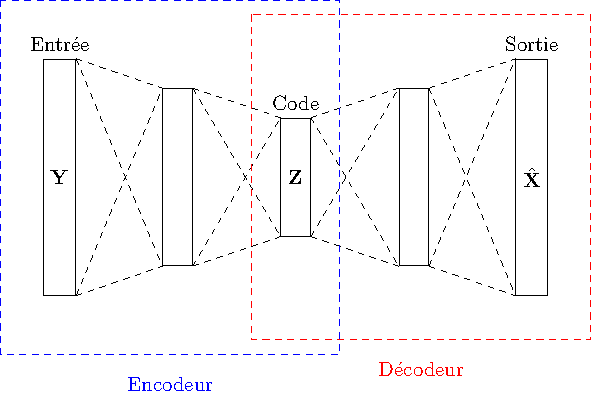
\includegraphics{img/chapitre2/figure6/denoising_deep.pdf}
    \caption{Illustration d'un auto-encodeur débruiteur. Après entraînement sur des données d'entraînement, l'observation corrompue \gls{Y} est fournie en entrée de l'encodeur afin d'extraire des variables latentes (ou code) caractéristiques de l'image. Un décodeur restitue ensuite une image corrigée \gls{Xh} à partir du code. Le réseau de neurone est dense.
        \protect\label{fig-denoising_deep}}
\end{figure}

Récemment, Ulyanov \etal~\cite{ulyanov2020deep} ont suggéré que les performances excellentes des réseaux de neurones, \ie\ leur capacité à capturer la statistique des images non-corrompues, ne sont pas dues à la phase d'entraînement et au large ensemble d'entraînement associé.
%
Au contraire, la structure du réseau seule serait suffisante à capturer la statistique des données, et cela, sans apprentissage. 
%
Les auteurs ont confirmé cette hypothèse en concevant un réseau génératif, défini par la fonction $f_\theta$ paramétrée par $\theta$, associant à un code $\mathbf{Z}$ une image $\gls{X}=f_\theta(\mathbf{Z})$. Après tirage d'un code aléatoire $\mathbf{Z}$, l'estimation de l'image reconstruite s'écrit donc
\begin{align}
    \hat{\theta} &= \argmin_\theta \frobnorm{\gls{Yi}-f_\theta(\mathbf{Z})_{\gls{I}}}\\
    \gls{Xh} &= f_{\hat{\theta}} (\mathbf{Z}).
\end{align}
En particulier, un réseau convolutif de type auto-encodeur a été utilisé par les auteurs. Cette implémentation affiche des performances supérieures aux autres méthodes par réseaux de neurones et indique que, pour extraire les caractéristiques de l'image à reconstruire, l'image corrompue seule est suffisante. Cette méthode n'a pas été utilisée dans ce manuscrit, faute de temps, mais elle demeure une perspective intéressante.


%We employ DA to perform pre-training in our method because it naturally lends itself to denoising
%and inpainting tasks. DA is a two-layer neural network that tries to reconstruct the original input
%from a noisy version of it. The structure of a DA is shown in Fig.1a. A series of DAs can be stacked
%to form a deep network called Stacked Denoising Auto-encoders (SDA) by using the hidden layer
%activation of the previous layer as input of the next layer.


%
\section{Utilisation des techniques de reconstruction en microscopie}\label{sec-art-micro}

La section précédente a présenté les différentes classes d'algorithmes employées dans la communauté du traitement du signal en vue de reconstruire des images spatialement sous-échantillonnées. Ces techniques ont fortement inspiré les travaux en microscopie visant à limiter la détérioration de l'échantillon en adoptant une approche par acquisition partielle, comme décrit à la \cref{sec-ech-sensibles}.
%
Ainsi, de nombreuses méthodes de reconstruction ont été proposées dans diverses modalités pour compléter l'acquisition partielle et certains travaux les ont comparés pour déterminer lesquelles privilégier.
%
D'autre part, puisque la qualité de reconstruction dépend significativement du chemin d'acquisition, divers travaux ont étudié le masque d'échantillonnage maximisant les performances pour un algorithme de reconstruction donné. Bien que seul le premier aspect ait été étudié dans le présent manuscrit, le second aspect est également d'un intérêt particulier et tous deux seront discutés.
%
La suite de cette section décrira les travaux de la communauté en microscopie traitant de ces aspects en dissociant les approches \emph{sans entraînement} ne nécessitant pas d'autre données que les seules données acquises et les approches \emph{avec entraînement} s'appuyant sur des données d'entraînement.

\subsection{Méthodes sans entraînement}

L'interpolation \gls{ppv} est une solution simple et rapide, autorisant parfois de réaliser conjointement l'acquisition et la reconstruction en temps réel. Cependant, pour éviter que l'image reconstruite soit constante par morceau, on préfère pondérer les valeurs prises par les pixels voisins, comme expliqué à l'\cref{eq-weighted-interp}. La distance entre le pixel à interpoler et le voisin est inversée puis normalisée afin de former la pondération. Cette approche est utilisée en reconstruction d'images \gls{sem} dans~\cite{godaliyadda2018tci}, \gls{edx} dans~\cite{zhang2018reduced, hujsak2018high} et \gls{eels} dans~\cite{hujsak2018high}. L'interpolation par plus proches voisins naturels qui ajuste les poids en se basant sur une représentation de Voronoi est choisie comme alternative pour des images \gls{sem} dans~\cite{trampert2018ultramicroscopy}.

Les méthodes par \gls{mc} régularisés offrent généralement de meilleurs résultats que \gls{ppv} puisqu'elles contraignent l'image reconstruite à suivre un comportement prédéfini, généralement au moyen d'une régularisation adaptée. Un choix classique puisque motivé par le paradigme de l'acquisition comprimée promeut la parcimonie dans une base adaptée, comme la régularisation $\ell_1$ utilisée pour des images de \gls{mfa} dans~\cite{han2018optimal}. Ce type de \gls{mc} régularisés sera noté $\ell_1-\mathrm{\gls{mc}}$ dans la \tabname~\ref{tab-litterature}. %
Dans le cas de structures périodiques (comme c'est le cas pour d'échantillons cristallins), la base de Fourier ou la \gls{dct} peuvent être utilisées. Les auteurs de~\cite{stevens2018apl} ont ainsi proposé une méthode de reconstruction d'image \gls{haadf} reposant sur une transformée de Fourier seuillée, contraignant ainsi la parcimonie dans cette base périodique. La méthode proposée dans~\cite{beche2016development} utilise l'algorithme SPGL1~\cite{berg2008probing} afin de promouvoir la parcimonie dans la base \gls{dct} et reconstruire des images \gls{haadf}. De la même façon, cette régularisation peut être couplée avec une base d'ondelettes pour reconstruire des images \gls{haadf} en ligne~\cite{li2018compressed}. %
%
La régularisation \gls{tv} est aussi classiquement utilisée pour favoriser la reconstruction d'images constantes par morceaux, comme proposé dans~\cite{han2018optimal} pour des données \gls{mfa}. La représentation \gls{dct} par bloc a été couplée avec la \gls{tv} en reconstruction d'images \gls{sem} dans~\cite{anderson2013sparse}.%



Les méthodes par patch offrent généralement de meilleurs performances puisqu'elles exploitent la redondance spatiale et apprennent un espace de représentation adaptée aux données. En particulier, les techniques par \gls{ad} estiment conjointement les atomes constituant un dictionnaire et la représentation parcimonieuse associée. %
%
L'algorithme BPFA est très probablement la méthode par \gls{ad} la plus populaire dans la communauté de microscopie~\cite{xing2012siam}. Elle a été appliquée pour la première fois sur des images \gls{haadf} à échelle atomique~\cite{stevens2014potential} et a été utilisée par la suite dans de nombreux travaux pour le même type de données~\cite{mucke2016practical,kovarik2016implementation}.
%
Les auteurs de BPFA ont également proposé la méthode Kruskal-factor analysis (KFA) comme une extension tensorielle de BPFA~\cite{stevens2017tensor}. KFA a été appliqué à la reconstruction d'images \gls{eels} en se basant sur une acquisition multiplexée d'un spectre-image~\cite{stevens2016mm}.
%
Enfin, l'algorithme expected-patch log-likelihood (EPLL) fait l'hypothèse que la distribution statistique des patchs suit un mélange de lois gaussiennes~\cite{zoran2011from}. Cependant, cet algorithme est particulièrement lent, si bien que les auteurs ont préféré une implémentation simplifiée mais accélérée appelée Fast EPLL (FEPLL) afin de reconstruire des images \gls{sem}~\cite{parameswaran2019accelerating}.
%
En plus des méthodes utilisées dans la communauté de microscopie, wKSVD~\cite{mairal2008tip} et ITKrMM~\cite{naumova2018fast,naumova2017dictionary} apprennent le dictionnaire à partir de données incomplètes sans faire d'hypothèse particulière sur la distribution des patchs. Il s'agit pourtant de méthodes de l'état de l'art et elles seront considérées dans la suite de l'étude.

Afin d'atteindre de meilleures performances avec une dose réduite d'électron, plusieurs chemins d'acquisition ont été proposés, comme l'échantillonnage aléatoire de lignes horizontales~\cite{kovarik2016implementation,han2018optimal}, l'échantillonnage mixe régulier-aléatoire~\cite{stevens2018apl}, les chemins en spirale~\cite{sang2017dynamic,li2018compressive,han2018optimal} ou enfin les chemins en forme de carré~\cite{han2018optimal}.
%
Ces résultats tendent à montrer que les performances optimales sont atteintes par des acquisitions semi-aléatoires, qui introduisent de l'aléatoire dans des structures régulières, ce qui évite les zones masquées de grande dimension. % 
%
Finalement, des améliorations conséquentes en reconstruction ont été rendues possibles par l'acquisition adaptative qui sélectionne le pixel à échantillonner à partir des données précédemment acquises. Dans~\cite{dahmen2016feature}, les auteurs proposent de faire un premier échantillonnage à bas \gls{snr} afin de localiser les contours de l'image. Une seconde acquisition à \gls{snr} élevé est ensuite effectuée sur ces contours seulement. Enfin, les parties lisses de la première image sont filtrées tandis que les contours sont remplis avec les pixels issus de la seconde acquisition. Un schéma d'acquisition adaptative alternatif proposé dans~\cite{dahmen2019adaptive} consiste à localiser de manière itérative des points d'intérêt à échantillonner. Les techniques d'acquisition adaptatives partielles avec entraînement sont présentées à la section suivante.

\subsection{Méthodes avec entraînement}

Contrairement aux méthodes sans apprentissage qui reconstruisent l'image complète à partir des seules données acquises, les méthodes avec entraînement apprennent un opérateur en exploitant des données d'entraînement. Par exemple, l'algorithme \gls{goal} apprend un dictionnaire en maximisant la parcimonie de la représentation des données d'apprentissage~\cite{hawe2013analysis}. Le dictionnaire estimé est ensuite utilisé afin de reconstruire les données de test. De manière similaire, \gls{ebi} qui est initialement une technique sans apprentissage peut être adapté afin de tirer parti de données d'apprentissage. Pour cela, au lieu d'extraire le patch à copier du voisinage, comme c'est le cas dans l'implémentation conventionnelle de \gls{ebi}, ce patch est choisi parmi un dictionnaire appris auparavant sur des images non-corrompues. Cette stratégie est suivie dans~\cite{trampert2018exemplar} pour reconstruire des données 3D en \gls{sem}. \gls{goal} et la version avec apprentissage de \gls{ebi} ont été appliqués dans~\cite{trampert2018ultramicroscopy} pour des images 2D en \gls{sem}, mais BPFA semblait donner de meilleurs résultats.

Les approches avec apprentissage peuvent aussi être envisagées afin de décider quelle position devrait être échantillonnée pour minimiser la distorsion après reconstruction. En effet, la position des pixels échantillonnés impacte grandement la qualité de la reconstruction lorsque les données sont sous-échantillonnées~\cite{trampert2018ultramicroscopy}. Pour améliorer cette qualité, l'algorithme SLADS (supervised learning approach for dynamic sampling) apprend une fonction (appelée réduction de distorsion espérée (RDE)) indiquant quelle position devrait être échantillonnée afin de réduire la distorsion au maximum~\cite{godaliyadda2018tci}. Cette étape d'apprentissage repose sur une liste de caractéristiques et sur des données labellisées et a été utilisée pour dynamiquement échantillonner des images \gls{sem}.
%
Cette méthode a aussi été appliquée à des données \gls{edx} dans~\cite{zhang2018reduced}. Pour cela, un réseau de neurones convolutif classe les spectres des données test et la fonction RDE est calculée simultanément pour toutes les classes. %
%
Le papier~\cite{hujsak2018high} a ensuite modifié cette approche pour permettre des mélanges d'éléments en \gls{eels} et en \gls{edx}. Toutes ces approches requièrent une technique de reconstruction rapide et l'interpolation pondérée \gls{ppv} a été utilisée.



%
\section{Contribution de la thèse}

\begin{mylandscape}
    \begin{normaltable}[]
        \centering
        \bgroup
    \renewcommand{\arraystretch}{1.2}
    \begin{tabular}{>{\arraybackslash\centering}m{3cm}*{5}{c}}
        \toprule
        \multirow{2}*{Famille}& \multirow{2}*{Méthode}& \multicolumn{2}{c}{Travaux}& 
        \multirow{2}*{Temps d'exécution}& \multirow{2}*{Précision}\\
        %
        &&2D&3D&&\\
        %
        \midrule
        %
        \multirow{2}*{Interpolation} & \gls{ppv} & - & - & \plusfa[3] & \minusfa[2]\\
        %
        & Voisinage pondéré & \cite{sibson1981interpreting, cazals2006delaunay, trampert2018ultramicroscopy}&
        - & \plusfa[2] & \minusfa[1]\\
        %
        \midrule
        %
        \multirow{2}*{\gls{mc} régularisés}&
        $\ell_1$-\gls{mc} & \cite{han2018optimal,beche2016development,li2018compressed,anderson2013sparse}& -
        & \plusfa & \plusfa\\
        %
        & TV-\gls{mc} & \cite{han2018optimal} & - & \plusfa[1] & \plusfa\\
        %
        %
        \midrule
        %
        \multirow{6}{3cm}{\centering Méthode par \gls{ad}}&
        BPFA & {\cite{stevens2014potential,trampert2018ultramicroscopy}} &
        \textit{\cite{xing2012siam}} & \minusfa[3] & \plusfa[3]\\
        %
        & EBI & \cite{trampert2018ultramicroscopy} & {\cite{trampert2018exemplar}} &
        \minusfa[1] & \plusfa[2]\\
        %
        & FEPLL & \textit{\cite{parameswaran2019accelerating}},\cite{hujsak2018high} &
        - & \minusfa[1] & \plusfa[2]\\
        %
        & wKSVD & - & \textit{\cite{mairal2008tip}} & \minusfa[2] & \plusfa[2]\\
        %
        &
        ITKrMM & \textit{\cite{naumova2018fast}} & \textit{\cite{naumova2017dictionary}}&
        \minusfa[1] & \plusfa[2]\\
        %
        & GOAL & \textit{\cite{hawe2013analysis}},\cite{trampert2018ultramicroscopy}&
        - & \minusfa[1] & \plusfa[2]\\
        %
        \bottomrule
    \end{tabular}
    \egroup
        \caption{Comparaison des méthodes proposées dans la littérature en microscopie pour le reconstruction d'images partiellement échantillonnées. Des références supplémentaires n'étant pas issues de la littérature en microscopie sont données en italique. Le temps d'exécution et la précision sont évaluées qualitativement en se basant sur les résultats des chapitres suivants.%
            \protect\label{tab-litterature}}
    \end{normaltable}
\end{mylandscape}

Dans cette étude, j'étudie des méthodes de reconstruction rapide pour les données \gls{stem}-\gls{eels} acquises partiellement. En particulier, une motivation consiste à réduire le temps de calcul associé à l'étape d'inpainting en vue de l'insérer dans le processus d'acquisition. L'expérimentateur devrait être capable de visualiser le spectre-image complet au cours de l'acquisition en vue de stopper prématurément l'échantillonnage si la zone ne se révèle pas intéressante, ce qui permettrait de préserver l'échantillon. Cela requiert à la fois un temps de calcul réduit et une bonne précision. En plus de ce processus dynamique, l'expérimentateur devrait être capable de raffiner le spectre-image reconstruit a posteriori. Dans ces conditions, des algorithmes plus performants mais nécessitant plus de temps de calcul pourront être utilisés. 


Afin de déterminer l'approche à privilégier, la \tabname~\ref{tab-litterature} résume l'état de l'art en microscopie réalisé dans la section précédente. Les méthodes y sont notées en fonction de leur complexité et de leurs performances et groupées selon trois grandes familles : l'interpolation, les \gls{mc} regularisés et les méthodes par \gls{ad}. Pour chaque méthode, les travaux issus de la littérature sont fournis et séparés selon que les données reconstruites soient des images 2D mono-bandes (\eg{} \gls{haadf}) ou des spectre-images 3D (\eg{} \gls{eels}).

Parmi les méthodes compatibles avec les données \gls{eels}, \gls{ppv} est rapide mais les performances en reconstruction sont généralement mauvaises tandis que les méthodes par \gls{ad} sont très efficaces mais sont très lourdes en temps de calcul, tout particulièrement lorsque des patchs 3D sont appris. Par conséquent, cet état de l'art met en évidence une lacune : aucune technique n'est disponible pour reconstruire précisément un spectre-image spatialement sous-échantillonné suffisamment rapidement pour l'inclure dans un processus expérimental d'acquisition en ligne. D'autant que l'acquisition et la reconstruction rapide d'un spectre-image \gls{eels} n'a suscité que peu d'intérêt en comparaison de sa contrepartie hyperspectrale en observation de la Terre~\cite{zhang_hyperspectral_2014, chayes_pre_processing_2017, golbabaee_hyperspectral_2012, chen_inpainting_2012}.

Une alternative pour systématiquement reconstruire un spectre-image consiste à traiter les images 2D associées à chaque canal \emph{séparément} et \emph{en parallèle}. Notons d'ailleurs que \gls{ppv} fonctionne de cette façon lorsqu'il reconstruit un spectre-image spatialement sous-échantillonné. Cependant, cette approche est sous-optimale : la tâche de reconstruction est censée être plus efficace en s'appuyant sur les données 3D complètes puisque les bandes du spectre-image sont corrélées. Des stratégies similaires consisteraient à ne reconstruire que les images associées à un ou plusieurs canaux d'intérêt nécessaires pour la cartographie d'éléments. Cependant, cette approche serait aussi sous-optimale quand aucun a priori serait disponible concernant l'échantillon à observer.

Pour conclure, ni l'interpolation \gls{ppv}, ni les méthodes par \gls{ad} ne sont adaptées à la reconstruction précise en ligne et seulement les méthodes par \gls{mc} allient précision et charge calculatoire réduite. C'est donc ce type d'approche qui a été étudié dans la suite de ce manuscrit. Et puisque les performances des méthodes par \gls{mc} régularisés dépendent fortement de l'information disponible a priori, la reconstruction d'images \gls{eels} spatialement lisses sera étudiée dans le \cref{ch-chapter_3} tandis que les échantillons cristallins le seront dans le \cref{ch-chapter_4}. Remarquons finalement que les méthodes par \gls{ad} sont les techniques les plus performantes disponibles et qu'elles conviennent parfaitement à l'étape de raffinement effectuée a posteriori. Le but poursuivi n'est pas de battre ces méthodes en termes de performance, mais de proposer des techniques efficaces ayant une faible charge calculatoire.  Ces méthodes particulièrement performantes ne seront pas étudiées par la suite et ne servirons que de comparaison aux approches proposées. 

